Ein Lock-In-Verstärker besteht aus einem Bandpassfilter, einem Phasenschieber
und einem Tiefpassfilter. Das eingehende, rauschende Signal $U_{sig}$ mit der Freqenz
$\omega_0$ wird vom Bandpassfilter
von hohen $(\omega \gg \omega_0)$ und tiefen $(\omega \ll \omega_0)$ Frequenzen befreit.
\\Durch den Phasenschieber wird die Spannung $U_{ref}$ auf die geeignete Phase gebracht ($\Delta\varphi=0$).
\\Am Mischer werden die beiden Signale multipliziert.
\\Anschließend dient ein Tiefpassfilter ($\tau = RC \gg \frac{1}{\omega_0}$) als Integrator des Mischsignals ($U_{sig}\times U_{ref}$).
Die Rauschbeträge werden bei dem Vorgang weitestgehend herausgemittelt.
\\Als Ausgangsspannung ergibt sich dann $U_{out}\propto U_0 \cos{\varphi}$.
Durch ein große Zeitkonstante $\tau = RC$ erreicht man, dass man den Bandpass beliebig klein machen kann.
So kann eine Güte von $Q = 100000$ erreicht werden. Ein einzelner Bandpass erreicht eine Güte von $Q = 1000$.
  \begin{figure}[h!]
    \centering
    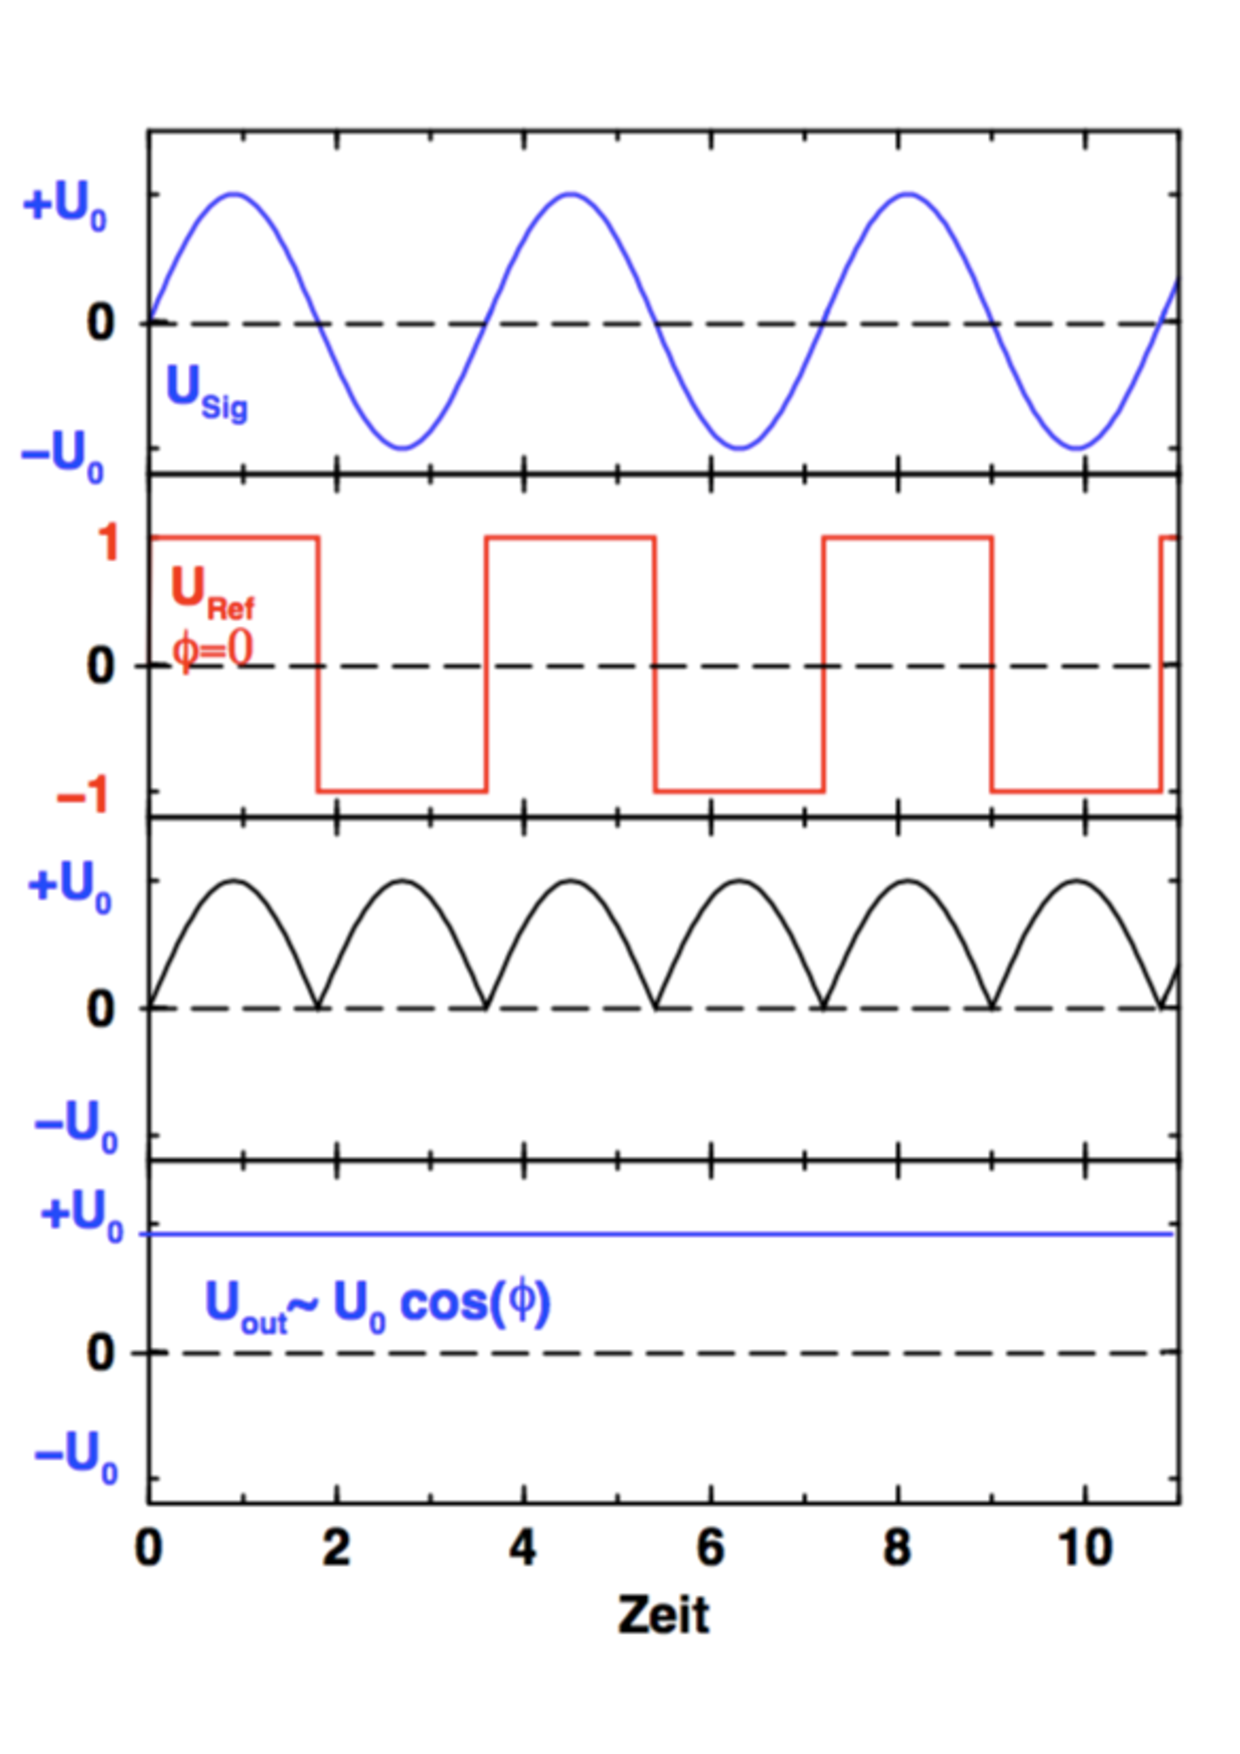
\includegraphics[width=0.8\textwidth]{Spannungen.pdf}
    \caption{Signalverläufe \cite{1}}
    \label{fig:sig}
  \end{figure}
\\In der Abbildung \ref{fig:sig} ist ein Signalverlauf einer Sinusspannung dargestellt($U_{sig} = U_0sin(\omega t)$).
Diese wird durch einen auf 1 normierte Rechteckspannung der selben Freqenz moduliert.
Durch eine Fourierreihe kann die Rechteckspannung angenähert werden.
Dabei werden nur die ungraden harmonischen Grundfreqenzen \omega genutzt.
\begin{equation}
  U_{ref} =  \frac{4}{\pi}  \left( \sin{\omega t}+\frac{1}{3}\sin{3\omega t}+\frac{1}{5}\sin{5\omega t}+...\right)
\end{equation}
\label{eqn:uref}
\\Für das Produkt aus Signal- und Modulationsfreqenz werden nun die graden Oberwellen der Grundfrequenz \omega benutzt. Daraus ergibt sich:
\begin{equation}
  U_{sig} \times U_{ref} =  \frac{2}{\pi}U_0  \left(1- \frac{2}{3}\cos{2\omega t}-\frac{2}{15}\cos{4\omega t}-\frac{2}{35}\cos{6\omega t}+...\right)
\end{equation}
\label{eqn:usig*uref}
\\Die Oberwellen werden wiederum vom nachgeschalteten Tiefpass unterdrückt. Daraus ergibt sich eine Gleichspannung welches proportional zum Eingangssignal ist.
\begin{equation}
  U_{out} =  \frac{2}{\pi}U_0 \cos{\varphi}.
\end{equation}
\label{eqn:uoutcos}
\\Sind $U_{sig}$ und $U_{ref}$ in Phase, also
\begin{equation*}
  \varphi = 0,
\end{equation*}
\\ergibt sich
\begin{equation}
  U_{out} =  \frac{2}{\pi}U_0.
\end{equation}
\label{eqn:uout}
\FloatBarrier
